\section{Experimento 1: Red de Starbucks}

\subsection{Descripción del contexto}

El experimento fue realizado en una red de FibertelZone, por medio de una conexión Wi-Fi en un local de Starbucks de Corrientes y Malabia. Dentro de la red se encuentran conectadas aproximadamente 10 notebooks y muchos celulares, además del router. La fecha de captura es Lunes 9 de Octubre de 2017.

\subsection{Descripción de la captura}

Capturamos 12000 paquetes. En la figura~\ref{protocolos1} se muestra la distribución de los protocolos en la red. Observamos que la mayoría de los paquetes son de tipo IPv4, otros son de tipo \texttt{0x86dd} (IPv6) y la minoría son de ARP.

Los paquetes de tipo IPv4 e IPv6 usan distintas versiones del protocolo IP. Los paquetes de tipo ARP son los usados por los hosts de una red para obtener direcciones MAC de otros dispositivos, a partir de su IP.

Esto es consistente, ya que la mayoría de los dispositivos usan IPv4/IPv6 para conectarse a Internet, y el porcentaje de paquetes ARP es considerable al haber muchos dispositivos conectados al mismo tiempo.

\begin{figure}[H]
\centering
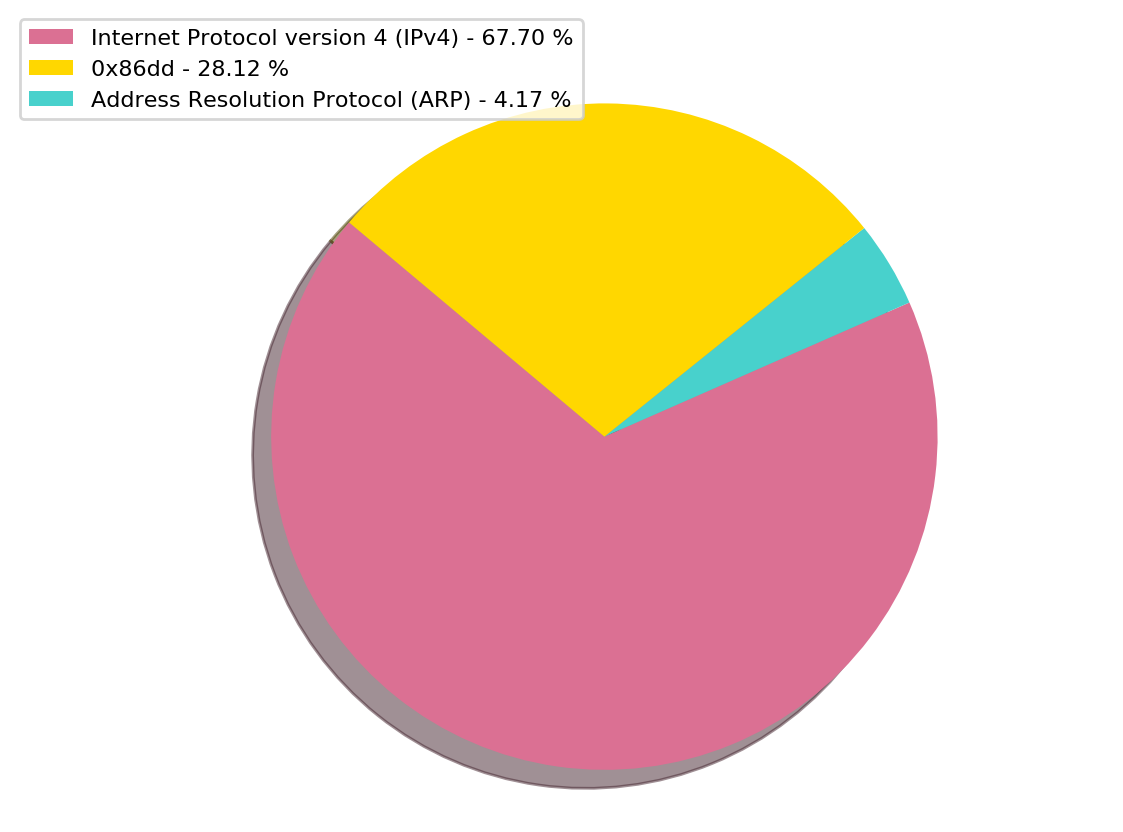
\includegraphics[width=0.7\textwidth]{protocolosRed1.png}
\caption{Gráfico que muestra la distribución de protocolos en la red.}
\label{protocolos1}
\end{figure}

En la figura~\ref{broadcast1} podemos ver el porcentaje de paquetes broadcast comparado con el total de paquetes. Vemos que esto representa un 16\% del total. En la figura~\ref{entropias1_1} vemos que los protocolos que aparecen en los paquetes de broadcast son ARP e IPv4. En cuanto a ARP, estos paquetes son los del tipo who-is, que mediante broadcast llegan al nodo cuya IP busca el emisor. 

\begin{figure}[H]
\centering
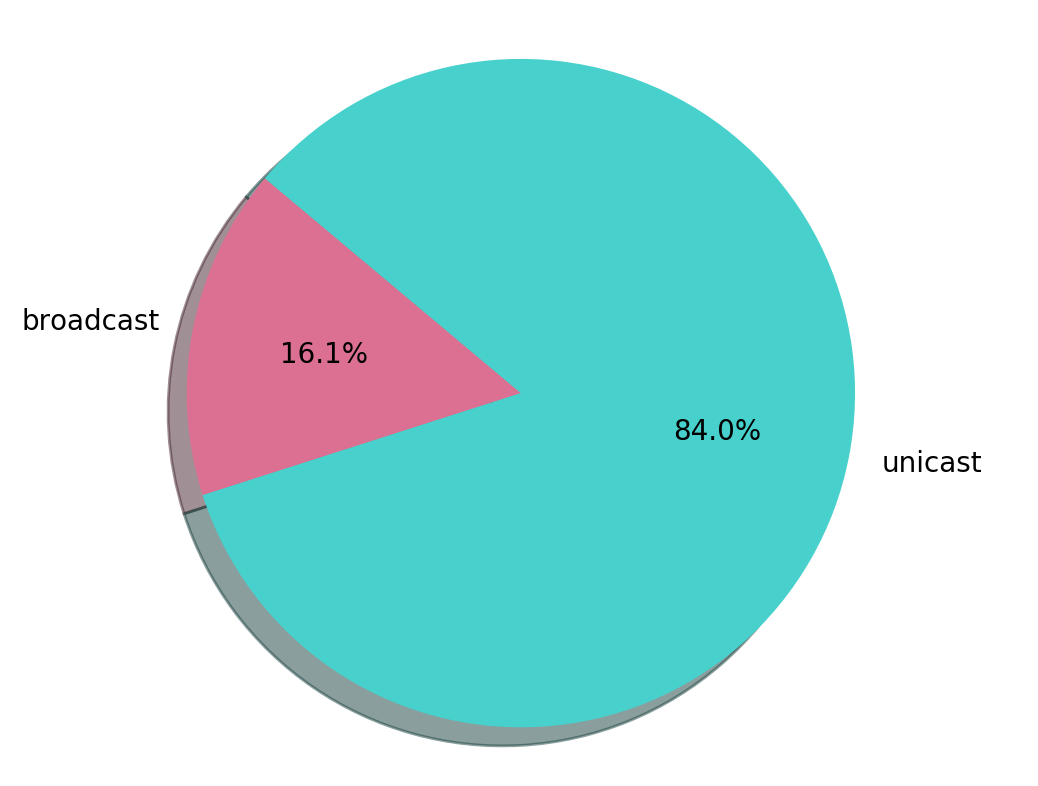
\includegraphics[width=0.7\textwidth]{broadcastRed1.png}
\caption{Gráfico que muestra los porcentajes de tráfico broadcast y unicast.}
\label{broadcast1}
\end{figure}

\subsection{Análisis de la captura}

Realizamos el modelado de la fuente $S_1$ según el enunciado. En la figura~\ref{entropias1_1} se encuentra el gráfico de la información de cada símbolo. Cuanta más información tenga un símbolo, quiere decir que es menos probable que aparezca. En esta red particular el símbolo con más información es representado por los paquetes unicast de tipo ARP. Estos paquetes son los is-at, las respuestas a los who-has. Tiene sentido ya que mientras que el request de ARP se hace mediante broadcast (o sea, mandando muchos paquetes), el reply es unicast (menos paquetes).

Además vemos que la entropía muestral es más de la mitad de la entropía máxima, esto es así porque la información de los distintos símbolos es comparable. El símbolo con más información (ARP, unicast) tiene aproximadamente 10 veces la información del menor (IPv4, unicast). La entropía máxima se alcanzaría si la información de todos los símbolos fuese la misma.

\begin{figure}[H]
\centering
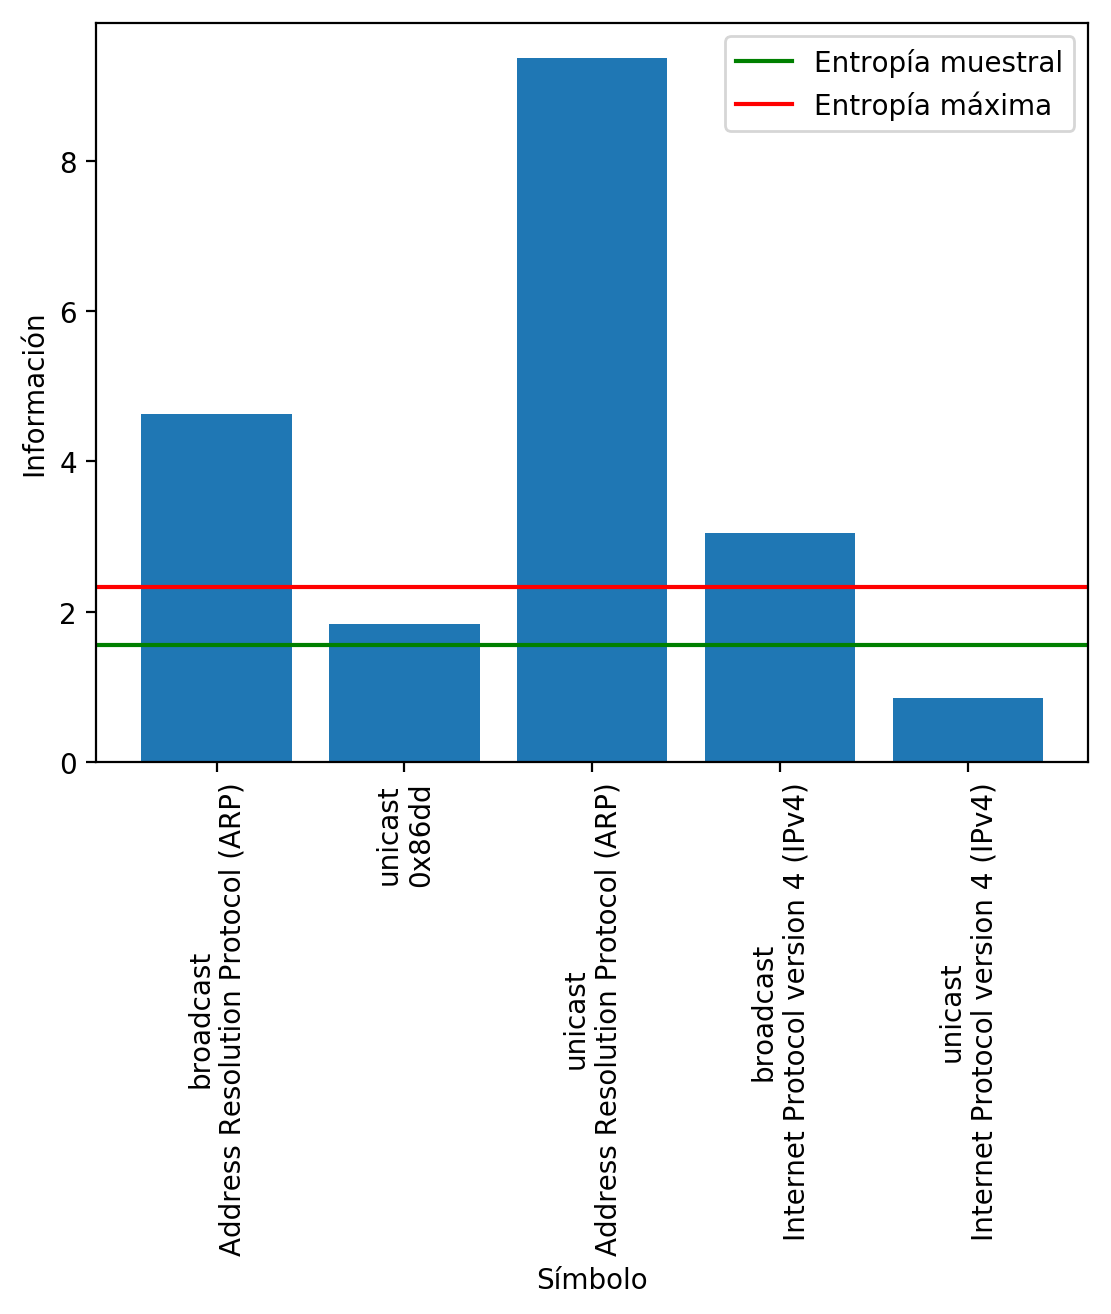
\includegraphics[width=0.7\textwidth]{entropiaS1Red1.png}
\caption{Gráfico de la información de los símbolos de la fuente $S_1$ observados en esta red. Se muestra la entropía muestral de $S_1$ y su entropía máxima.}
\label{entropias1_1}
\end{figure}

El análisis usando el modelado de la fuente $S_2$ (explicado anteriormente) se puede ver en la figura~\ref{entropias2_1}. En este caso vemos que los símbolos de la fuente podrían dividirse en 2 o 3 grupos de acuerdo a su información. Se observan algunos puntos distinguidos, en particular las 8 IPs con información menor a la entropía de $S_2$. Estas son las IPs que más requests de ARP hicieron. 

La entropía muestral es aproximadamente $\frac{4}{5}$ de la máxima. Es alta ya que hay muchos símbolos con valores parecidos de información; la máxima se alcanzaría con equiprobabilidad.

\begin{figure}[H]
\centering
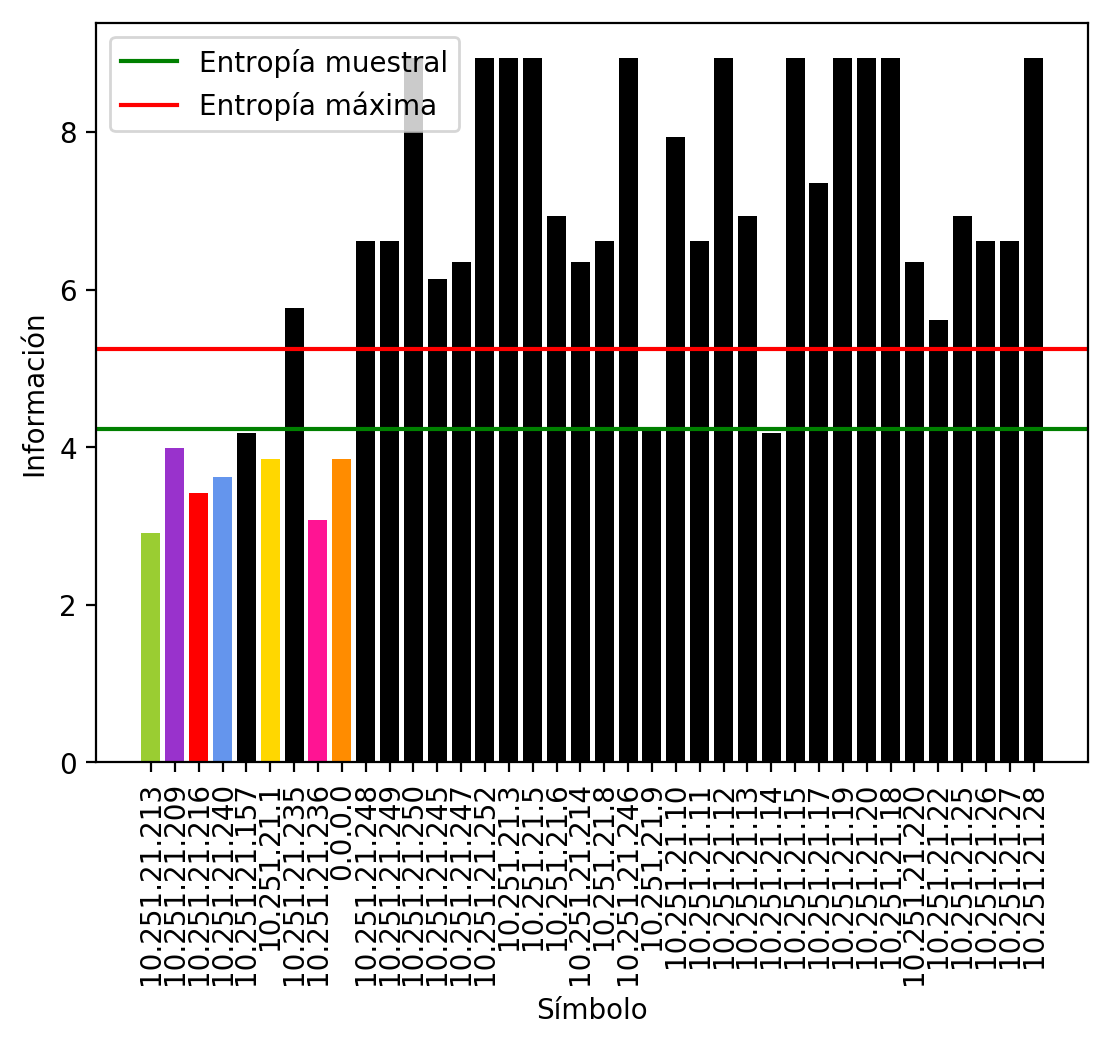
\includegraphics[width=0.7\textwidth]{entropiaS2Red1.png}
\caption{Gráfico de la información de los símbolos de la fuente $S_2$ observados en esta red. Se muestra la entropía muestral de $S_2$ y su entropía máxima.}
\label{entropias2_1}
\end{figure}

Por último graficamos la red subyacente de mensajes ARP, en la figura~\ref{grafo1}. Cada nodo del grafo representa una IP interviniente en al menos un mensaje ARP de la red, y cada eje orientado representa que la primera IP envió al menos un mensaje a la segunda. No estamos distinguiendo entre paquetes de tipo who-has o is-at. Podemos ver que el nodo central se comunica separadamente con muchos otros nodos, por lo que creemos que es el router del Stabucks.

\begin{figure}[H]
\centering
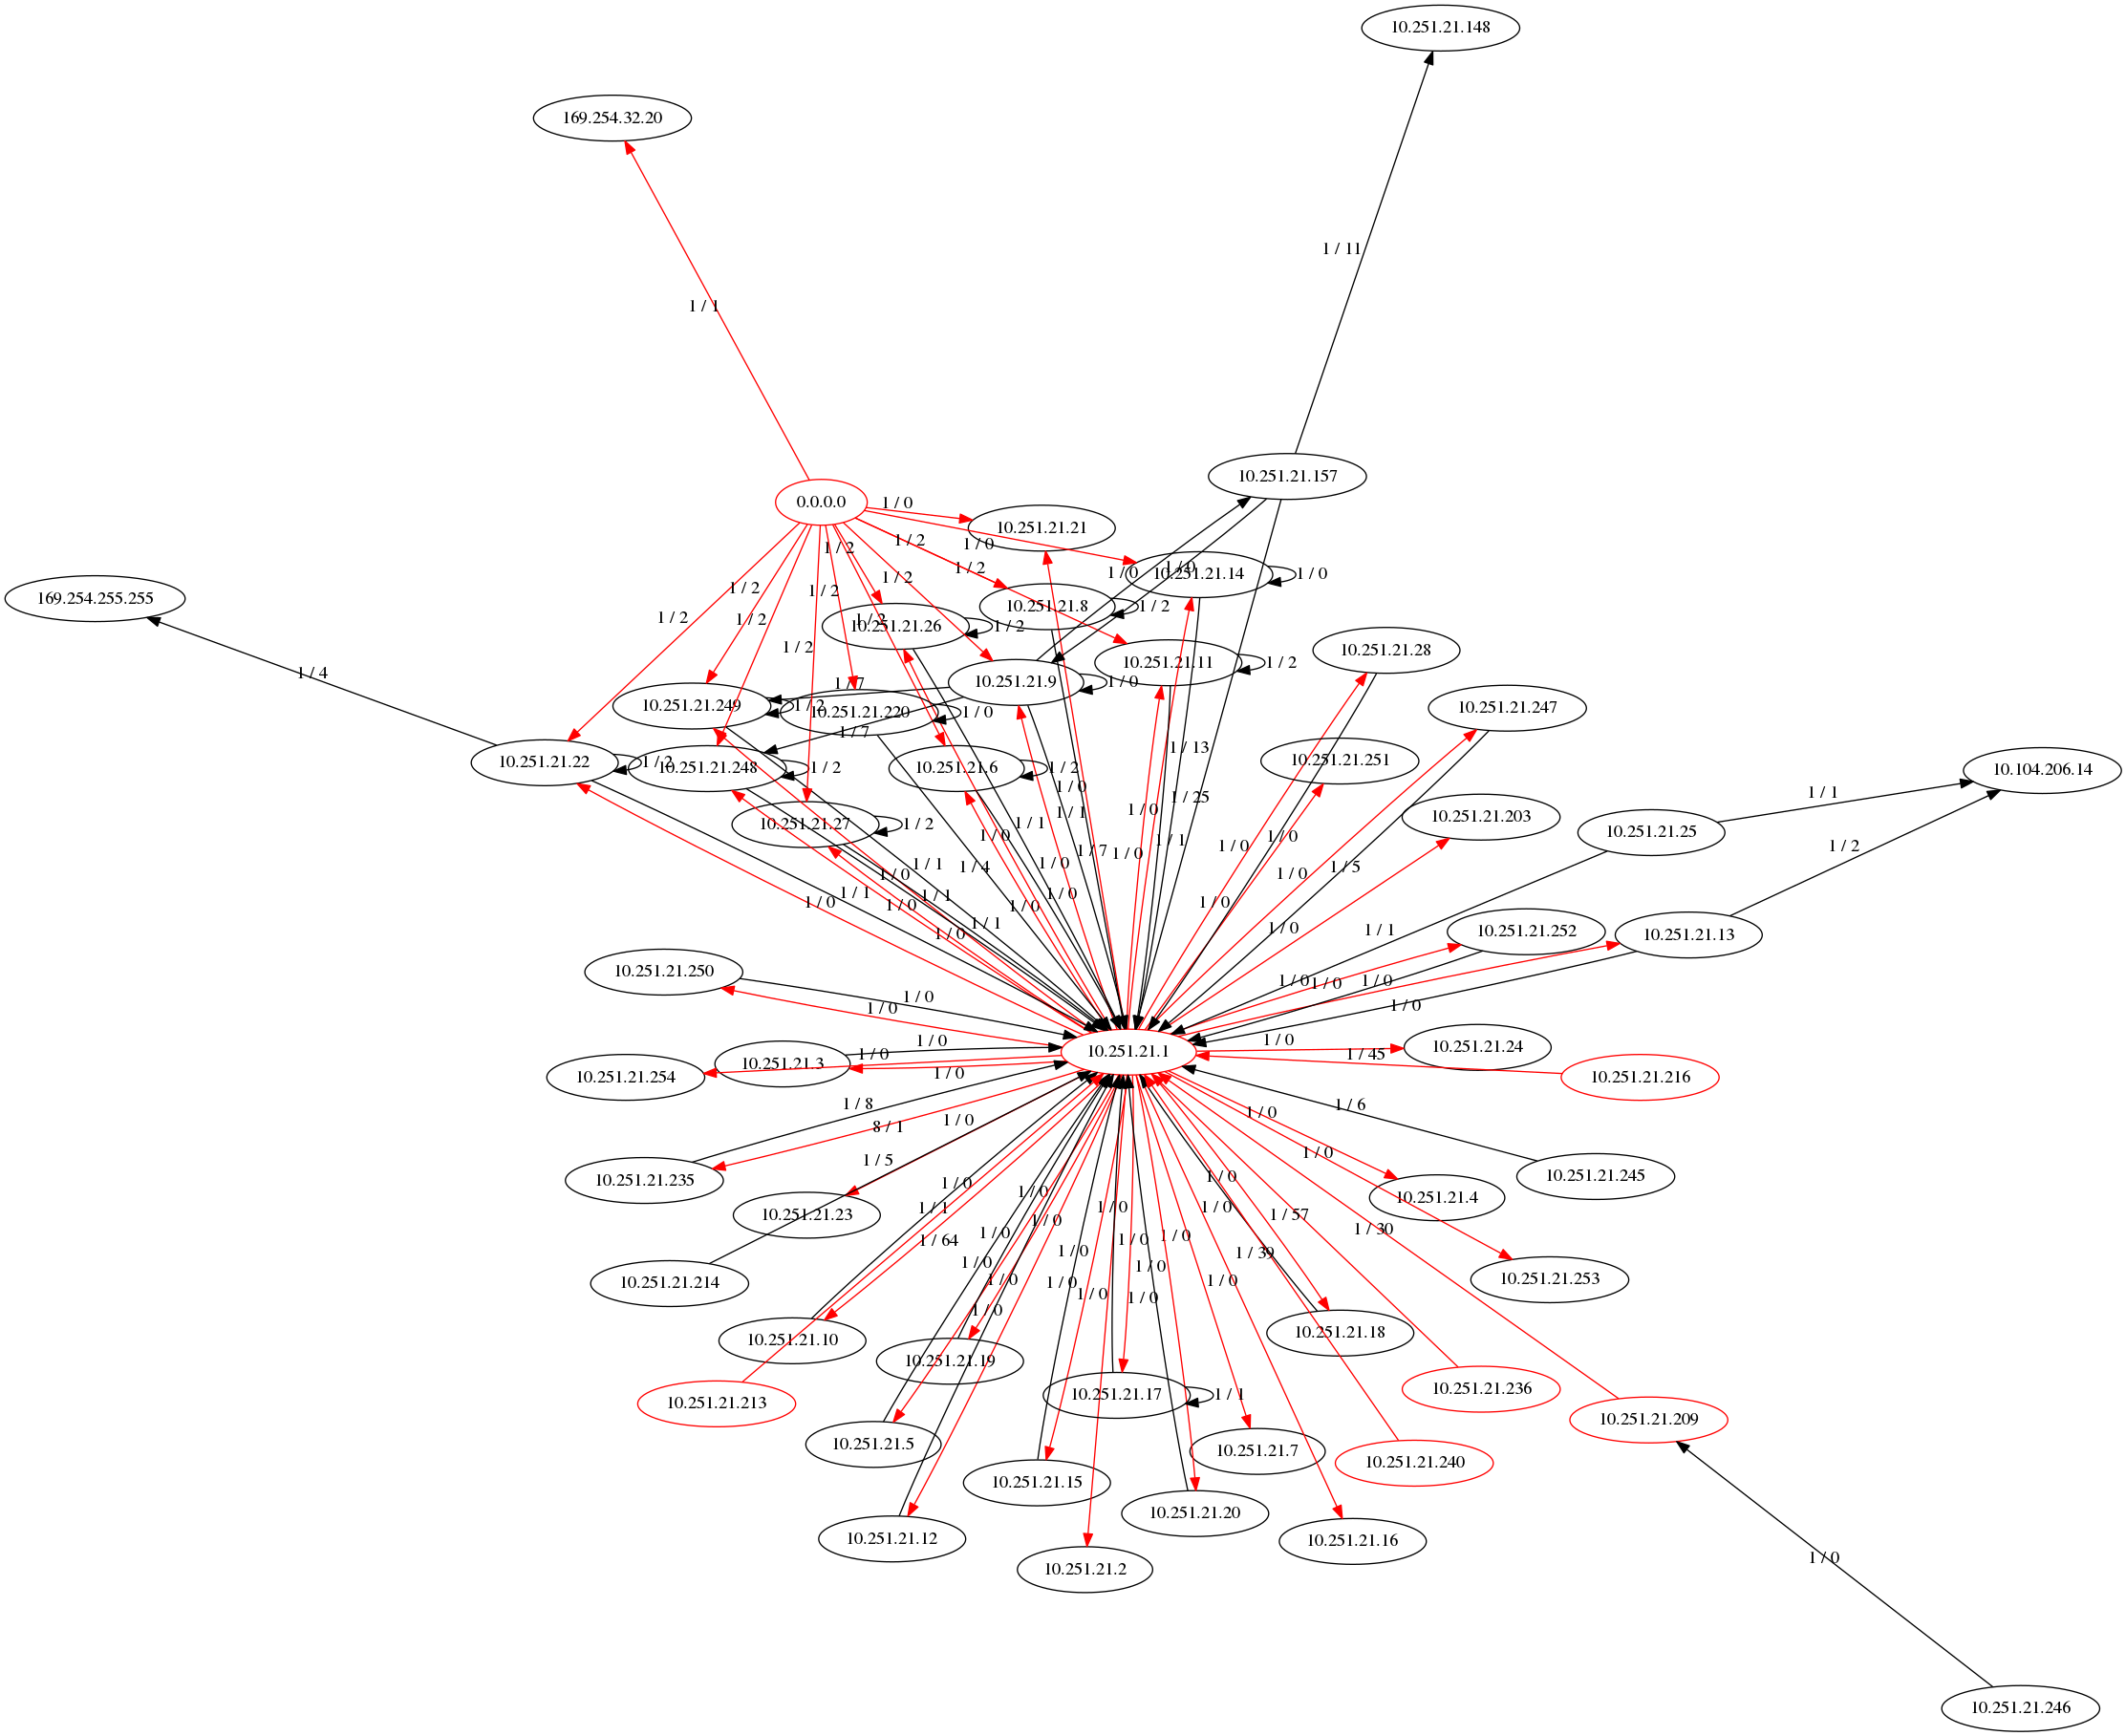
\includegraphics[width=\textwidth]{grafoRed1.png}
\caption{Grafo de la red de mensajes ARP subyacente. Los nodos son las IPs observadas y los ejes son los mensajes ARP. En colores se marcan los nodos distinguidos (información por debajo de la entropía) y sus mensajes salientes. Cada arista tiene anotada la cantidad de requests/replies ARP.}
\label{grafo1}
\end{figure}
